% Paper 3: skeleton (generation 68). Chapters 1 to 7 have text (generation 69); Chapters 8, 9
% and the appendix (generation 70).
% Decided (generation 83, S29 to S33): the subtitle, the author line, the chapter order, the titles.
% Material: Backlog items 5, 10, 11, 17; the History (B1, generation 67; A, generation 68).
% Every Lean name below was checked against the tree in generation 68.
% Preamble: paper 2's, without its figures (generation 68).
\documentclass[10pt,a4paper,titlepage]{article}
\usepackage[utf8]{inputenc}
\usepackage{amsmath,amssymb,amsthm}
\usepackage[margin=1.25in]{geometry}
% References into papers 1 and 2: their .aux files are read, the links go to their PDFs
\usepackage{xr-hyper}
\externaldocument[P1-]{R_collatz_stop_at_the_drop_1}[R_collatz_stop_at_the_drop_1.pdf]
\externaldocument[P2-]{R_collatz_stop_at_the_drop_2}[R_collatz_stop_at_the_drop_2.pdf]
\usepackage{hyperref}
\hypersetup{colorlinks, allcolors=blue!50!black}
% Index: the entry of a key term links to the passage that introduces the term
\makeatletter
\newcommand{\termhere}[1]{\leavevmode
  \Hy@raisedlink{\hyper@anchorstart{term:#1}\hyper@anchorend}}
\newcommand{\boxhere}[1]{\leavevmode
  \Hy@raisedlink{\hyper@anchorstart{box:#1}\hyper@anchorend}}
\makeatother
\newcommand{\termlink}[2]{\hyperlink{term:#1}{#2}}
% A key term where it is introduced: italic, with a link to its entry in the box
% of its chapter (\boxhere)
\newcommand{\keyterm}[2]{\hyperlink{box:#1}{\emph{#2}}}
% A symbol that is a key term, where its meaning is given: the same link, no italics
\newcommand{\keysym}[2]{\hyperlink{box:#1}{#2}}
\usepackage{booktabs}
\usepackage{array}
\usepackage{xcolor}
\usepackage{tikz}
\definecolor{chordblue}{HTML}{2A78D6}
\definecolor{chordorange}{HTML}{EB6834}
\usepackage{etoolbox}
\IfFileExists{imakeidx.sty}
  {\usepackage{imakeidx}\makeindex[intoc]}
  {\usepackage{makeidx}\makeindex}

% Layout: paper (default) or screen: pdflatex "\def\screenversion{}\input{file}"
\newif\ifpaper
\papertrue
\ifdefined\screenversion \paperfalse \fi

% Lean declaration and pv.py command
\newcommand{\lean}[1]{\textsf{#1}}
\newcommand{\pv}[1]{\texttt{pv.py #1}}
% number in binary
\newcommand{\bin}[1]{\text{\texttt{#1}}_2}
\ExplSyntaxOn
\seq_new:N \l__bw_parts_seq
\bool_new:N \l__bw_first_bool
\cs_new_protected:Npn \__bw_part:n #1
  {
    \fcolorbox{black!50}{black!5}
      {
        \bool_set_true:N \l__bw_first_bool
        \tl_map_inline:nn {#1}
          {
            \bool_if:NF \l__bw_first_bool { \textcolor{black!30}{\vrule width 0.3pt} }
            \bool_set_false:N \l__bw_first_bool
            \makebox[0.62em]{\rule[-0.4ex]{0pt}{2.2ex}\ttfamily ##1}
          }
      }
  }
% binary word: digits in cells, parts split at "-"
\NewDocumentCommand \bw { m }
  {
    \text
      {
        \group_begin:
        \setlength{\fboxsep}{0pt}
        \setlength{\fboxrule}{0.4pt}
        \seq_set_split:Nnn \l__bw_parts_seq { - } {#1}
        \seq_map_indexed_inline:Nn \l__bw_parts_seq
          {
            \int_compare:nNnF {##1} = {1} { \hspace{0.1em}\texttt{-}\hspace{0.1em} }
            \__bw_part:n {##2}
          }
        \group_end:
      }
  }
\ExplSyntaxOff
% Words without frames: pdflatex "\def\plainwords{}\input{file}"
\ifdefined\plainwords \RenewDocumentCommand \bw { m } {\text{\texttt{#1}}} \fi
\usepackage{listings}
\lstset{basicstyle=\ttfamily\small, columns=fullflexible, keepspaces=true}

% Glossary box at the end of each chapter
\newsavebox{\wordboxbin}
\newenvironment{wordbox}
  {\par\ifpaper\vspace*{\fill}\vspace{\bigskipamount}\else\medskip\fi
   \noindent\begin{lrbox}{\wordboxbin}%
   \begin{minipage}{\dimexpr\linewidth-6pt-2\fboxrule\relax}\small
   \begin{tabular}{@{}>{\bfseries\boldmath\raggedright\arraybackslash}p{0.24\linewidth}p{0.68\linewidth}@{}}}
  {\end{tabular}\end{minipage}\end{lrbox}%
   \begingroup\setlength{\fboxsep}{0pt}%
   \fcolorbox{black!40}{black!5}{\begin{minipage}{\dimexpr\linewidth-2\fboxrule\relax}%
     {\setlength{\fboxsep}{3pt}\colorbox{black!18}{\makebox[\dimexpr\linewidth-6pt\relax][l]%
       {\small\bfseries\strut Key terms introduced in Chapter~\thesection}}}\par\nointerlineskip
     {\color{black!40}\rule{\linewidth}{0.4pt}}\par\nointerlineskip
     \vspace{3pt}\noindent\hspace*{3pt}\usebox{\wordboxbin}\par\vspace{3pt}%
   \end{minipage}}\endgroup\par\ifpaper\else\medskip\fi}

% A figure or table set where it stands, on one page with what follows it
\makeatletter
\newenvironment{herefloat}[1]
  {\par\addvspace{\intextsep}\noindent\begin{minipage}{\linewidth}%
   \def\@captype{#1}\centering}
  {\end{minipage}\par\nopagebreak\vspace{\intextsep}}
\makeatother

% the first word of Order 5 as a staircase on the slanted grid, generated by stair_fig.py
\newcommand{\staircasefig}{%
  \draw[darkgray, line width=0.4pt] (0.000,-0.000) -- (12.918,-5.670);
  \node[anchor=base, font=\footnotesize] at (0.000,0.743) {$j=0$};
  \draw[gray, line width=0.4pt] (1.552,-0.000) -- (12.758,-4.918);
  \node[anchor=base, font=\footnotesize] at (1.552,0.743) {$j=1$};
  \draw[gray, line width=0.4pt] (3.105,-0.000) -- (12.758,-4.237);
  \node[anchor=base, font=\footnotesize] at (3.105,0.743) {$j=2$};
  \draw[gray, line width=0.4pt] (4.657,-0.000) -- (12.758,-3.555);
  \node[anchor=base, font=\footnotesize] at (4.657,0.743) {$j=3$};
  \draw[gray, line width=0.4pt] (6.210,-0.000) -- (12.758,-2.874);
  \node[anchor=base, font=\footnotesize] at (6.210,0.743) {$j=4$};
  \draw[gray, line width=0.4pt] (7.763,-0.000) -- (12.758,-2.192);
  \node[anchor=base, font=\footnotesize] at (7.763,0.743) {$j=5$};
  \draw[gray, line width=0.4pt] (9.315,-0.000) -- (12.758,-1.511);
  \node[anchor=base, font=\footnotesize] at (9.315,0.743) {$j=6$};
  \draw[gray, line width=0.4pt] (10.867,-0.000) -- (12.758,-0.830);
  \node[anchor=base, font=\footnotesize] at (10.867,0.743) {$j=7$};
  \draw[gray, line width=0.4pt] (12.420,-0.000) -- (12.758,-0.148);
  \node[anchor=base, font=\footnotesize] at (12.420,0.743) {$j=8$};
  \draw[darkgray, line width=0.4pt] (0.000,-0.000) -- (12.758,-0.000);
  \node[left, font=\footnotesize] at (-0.405,-0.000) {$i=0$};
  \draw[gray, line width=0.4pt] (2.461,-1.080) -- (12.758,-1.080);
  \node[left, font=\footnotesize] at (-0.405,-1.080) {$i=1$};
  \draw[gray, line width=0.4pt] (4.921,-2.160) -- (12.758,-2.160);
  \node[left, font=\footnotesize] at (-0.405,-2.160) {$i=2$};
  \draw[gray, line width=0.4pt] (7.382,-3.240) -- (12.758,-3.240);
  \node[left, font=\footnotesize] at (-0.405,-3.240) {$i=3$};
  \draw[gray, line width=0.4pt] (9.843,-4.320) -- (12.758,-4.320);
  \node[left, font=\footnotesize] at (-0.405,-4.320) {$i=4$};
  \draw[gray, line width=0.4pt] (12.303,-5.400) -- (12.758,-5.400);
  \node[left, font=\footnotesize] at (-0.405,-5.400) {$i=5$};
  \fill[darkgray] (0.000,-0.000) circle (1.5pt);
  \fill[darkgray] (1.552,-0.000) circle (1.5pt);
  \fill[darkgray] (3.105,-0.000) circle (1.5pt);
  \fill[darkgray] (4.657,-0.000) circle (1.5pt);
  \fill[darkgray] (6.210,-0.000) circle (1.5pt);
  \fill[darkgray] (7.763,-0.000) circle (1.5pt);
  \fill[darkgray] (9.315,-0.000) circle (1.5pt);
  \fill[darkgray] (10.867,-0.000) circle (1.5pt);
  \fill[darkgray] (12.420,-0.000) circle (1.5pt);
  \fill[darkgray] (2.461,-1.080) circle (1.5pt);
  \fill[darkgray] (4.013,-1.080) circle (1.5pt);
  \fill[darkgray] (5.566,-1.080) circle (1.5pt);
  \fill[darkgray] (7.118,-1.080) circle (1.5pt);
  \fill[darkgray] (8.671,-1.080) circle (1.5pt);
  \fill[darkgray] (10.223,-1.080) circle (1.5pt);
  \fill[darkgray] (11.776,-1.080) circle (1.5pt);
  \fill[darkgray] (4.921,-2.160) circle (1.5pt);
  \fill[darkgray] (6.474,-2.160) circle (1.5pt);
  \fill[darkgray] (8.026,-2.160) circle (1.5pt);
  \fill[darkgray] (9.579,-2.160) circle (1.5pt);
  \fill[darkgray] (11.131,-2.160) circle (1.5pt);
  \fill[darkgray] (7.382,-3.240) circle (1.5pt);
  \fill[darkgray] (8.934,-3.240) circle (1.5pt);
  \fill[darkgray] (10.487,-3.240) circle (1.5pt);
  \fill[darkgray] (12.039,-3.240) circle (1.5pt);
  \fill[darkgray] (9.843,-4.320) circle (1.5pt);
  \fill[darkgray] (11.395,-4.320) circle (1.5pt);
  \fill[darkgray] (12.303,-5.400) circle (1.5pt);
  \draw[chordorange, dashed, line width=0.8pt] (9.843,0.135) -- (9.843,-5.805);
  \node[below, font=\footnotesize] at (9.843,-5.805) {$3^{4} = 81$};
  \draw[chordblue, line width=1.2pt] (9.843,-4.320) -- (8.934,-3.240) -- (9.579,-2.160) -- (8.671,-1.080) -- (9.315,-0.000);
  \filldraw[draw=chordblue, fill=chordblue!35, line width=0.8pt] (9.843,-4.320) circle (3.8pt);
  \filldraw[draw=chordblue, fill=chordblue!35, line width=0.8pt] (8.934,-3.240) circle (3.8pt);
  \filldraw[draw=chordblue, fill=chordblue!35, line width=0.8pt] (9.579,-2.160) circle (3.8pt);
  \filldraw[draw=chordblue, fill=chordblue!35, line width=0.8pt] (8.671,-1.080) circle (3.8pt);
  \filldraw[draw=chordblue, fill=chordblue!35, line width=0.8pt] (9.315,-0.000) circle (3.8pt);
  \draw[chordorange, line width=1pt] (12.303,-5.400) circle (5pt);
  \draw[chordorange, line width=1pt] (12.420,-0.000) circle (5pt);
  \node[anchor=base, yshift=7pt, inner sep=0pt, font=\scriptsize, text=darkgray] at (0.000,-0.000) {$1$};
  \node[anchor=base, yshift=7pt, inner sep=0pt, font=\scriptsize, text=darkgray] at (1.552,-0.000) {$2$};
  \node[anchor=base, yshift=7pt, inner sep=0pt, font=\scriptsize, text=darkgray] at (3.105,-0.000) {$4$};
  \node[anchor=base, yshift=7pt, inner sep=0pt, font=\scriptsize, text=darkgray] at (4.657,-0.000) {$8$};
  \node[anchor=base, yshift=7pt, inner sep=0pt, font=\scriptsize, text=darkgray] at (6.210,-0.000) {$16$};
  \node[anchor=base, yshift=7pt, inner sep=0pt, font=\scriptsize, text=darkgray] at (7.763,-0.000) {$32$};
  \node[anchor=base, yshift=7pt, inner sep=0pt, font=\scriptsize, text=chordblue] at (9.315,-0.000) {$64$};
  \node[anchor=base, yshift=7pt, inner sep=0pt, font=\scriptsize, text=darkgray] at (10.867,-0.000) {$128$};
  \node[anchor=base, yshift=7pt, inner sep=0pt, font=\scriptsize, text=darkgray] (top) at (12.420,-0.000) {$256$};
  \node[anchor=base east, inner sep=0pt, font=\scriptsize, text=darkgray] at (top.base west) {$2^{8} = {}$};
  \node[anchor=north east, xshift=-1.5pt, yshift=-2.5pt, inner sep=0pt, font=\scriptsize, text=darkgray] at (2.461,-1.080) {$3$};
  \node[anchor=north east, xshift=-1.5pt, yshift=-2.5pt, inner sep=0pt, font=\scriptsize, text=darkgray] at (4.013,-1.080) {$6$};
  \node[anchor=north east, xshift=-1.5pt, yshift=-2.5pt, inner sep=0pt, font=\scriptsize, text=darkgray] at (5.566,-1.080) {$12$};
  \node[anchor=north east, xshift=-1.5pt, yshift=-2.5pt, inner sep=0pt, font=\scriptsize, text=darkgray] at (7.118,-1.080) {$24$};
  \node[anchor=north east, xshift=-4.5pt, yshift=-2pt, inner sep=0pt, font=\scriptsize, text=chordblue] at (8.671,-1.080) {$48$};
  \node[anchor=north east, xshift=-1.5pt, yshift=-2.5pt, inner sep=0pt, font=\scriptsize, text=darkgray] at (10.223,-1.080) {$96$};
  \node[anchor=north east, xshift=-1.5pt, yshift=-2.5pt, inner sep=0pt, font=\scriptsize, text=darkgray] at (11.776,-1.080) {$192$};
  \node[anchor=north east, xshift=-1.5pt, yshift=-2.5pt, inner sep=0pt, font=\scriptsize, text=darkgray] at (4.921,-2.160) {$9$};
  \node[anchor=north east, xshift=-1.5pt, yshift=-2.5pt, inner sep=0pt, font=\scriptsize, text=darkgray] at (6.474,-2.160) {$18$};
  \node[anchor=north east, xshift=-1.5pt, yshift=-2.5pt, inner sep=0pt, font=\scriptsize, text=darkgray] at (8.026,-2.160) {$36$};
  \node[anchor=north east, xshift=-4.5pt, yshift=-2pt, inner sep=0pt, font=\scriptsize, text=chordblue] at (9.579,-2.160) {$72$};
  \node[anchor=north east, xshift=-1.5pt, yshift=-2.5pt, inner sep=0pt, font=\scriptsize, text=darkgray] at (11.131,-2.160) {$144$};
  \node[anchor=north east, xshift=-1.5pt, yshift=-2.5pt, inner sep=0pt, font=\scriptsize, text=darkgray] at (7.382,-3.240) {$27$};
  \node[anchor=north east, xshift=-4.5pt, yshift=-2pt, inner sep=0pt, font=\scriptsize, text=chordblue] at (8.934,-3.240) {$54$};
  \node[anchor=north east, xshift=-1.5pt, yshift=-2.5pt, inner sep=0pt, font=\scriptsize, text=darkgray] at (10.487,-3.240) {$108$};
  \node[anchor=north east, xshift=-1.5pt, yshift=-2.5pt, inner sep=0pt, font=\scriptsize, text=darkgray] at (12.039,-3.240) {$216$};
  \node[anchor=north east, xshift=-4.5pt, yshift=-2pt, inner sep=0pt, font=\scriptsize, text=chordblue] at (9.843,-4.320) {$81$};
  \node[anchor=north east, xshift=-1.5pt, yshift=-2.5pt, inner sep=0pt, font=\scriptsize, text=darkgray] at (11.395,-4.320) {$162$};
  \node[anchor=north east, xshift=-5.5pt, yshift=-4pt, inner sep=0pt, font=\scriptsize, text=darkgray] at (12.303,-5.400) {$3^{5} = 243$};
}

\ifpaper\pretocmd{\section}{\clearpage}{}{}\fi
\newtheorem{theorem}{Theorem}
\emergencystretch=3em
% A float on a page of its own stands at the top
\makeatletter\setlength{\@fptop}{0pt}\makeatother
% Paragraphs are never split across pages (paper version)
\raggedbottom
\ifpaper
\interlinepenalty=10000
\postdisplaypenalty=10000
\fi

\title{\textbf{Collatz, but stop at the drop}\\[0.5ex]
  \Large The game on the grid of $2^j 3^i$}
\author{\textbf{Ruud H.G. van Tol}}
\date{\textbf{Draft: R\_84}}  % on the public site as a draft; no date (user, 28 Oct 2026)

\begin{document}
\maketitle

\section{One language for the drop and the 3-smooth numbers}
\label{sec:language}
% Generation 69: first text. Backlog 11. Papers 1 and 2 by reference (P1-, P2-).

Papers~1 and~2 study the drop: does every $x > 1$ eventually fall below itself under the
map $T$? Paper~2 reduces it to two open statements, the covering and the width identity
(paper~2, Chapter~\ref{P2-sec:open}). This paper collects what lies around them and is
proved, and some of what is measured, in one language: the grid of the numbers $2^j 3^i$.
\termhere{proved}\keyterm{proved}{Proved} means proved in Lean where a name is given;
\termhere{measured}\keyterm{measured}{measured} means computed exactly, on the range given.

\subsection*{One grid}

The $3$-smooth numbers are the points of the grid, sorted by their binary logarithm
$j + i\log_2 3$. The admissible words live on the same grid: the $n$ odd steps of a word of
Order $n$ are $n$ points, one per row, a staircase that starts at $3^{n-1}$ and stays to
its left (Chapter~\ref{sec:staircases}). The exact links between the two:
\begin{itemize}
\item $p_2(n)$, the length of a word of Order $n$, is the binary length of $3^n$, and the
  sum of the $p_2(k)$ is a term of Mintz's~\cite{Mintz1981} count of the $3$-smooth numbers below $2^j 3^i$
  (\lean{card\_smoothBelowAt}; paper~2, Chapter~\ref{P2-sec:chain}).
\item The record Orders of the block factor $f(n) = 3^n/2^{p_2(n)}$ decide the blocks of the
  chain of a word (paper~2), and also the step from a $3$-smooth number to the next
  (\lean{smooth\_next}, \lean{smooth\_succ}; Chapter~\ref{sec:staircases}).
\item $\rho$, the constant of $T^L(x) = (3^n x + \rho)/2^L$, is the sum of the staircase's
  $n$ points, and $d_{23}(n) = 2^{p_2(n)} - 3^n$ is a difference of two $3$-smooth numbers.
  The width identity says that the class id times this difference exceeds the sum of the
  staircase (\lean{ClassDrops}, \lean{widthIdentity\_iff\_classDrops}).
\end{itemize}
Whether this language moves either open statement is not known; it is a common language,
not yet a tool.

The Lean files, the scripts and this text were written with the assistance of Claude
(Anthropic) (Appendix~\ref{app:lean}); the author checked the statements and takes
responsibility for them.

\subsection*{The chapters}

Chapter~\ref{sec:staircases} draws the words as staircases and bounds $\rho$.
Chapter~\ref{sec:rhomax} takes the largest $\rho$ of each Order as the bound of the finite
reduction of the width identity, with its records. Chapter~\ref{sec:congruence} asks whether
the congruences that fix a class id carry the drop, and finds that they restate it.
Chapter~\ref{sec:a003586} finds the $n$-th $3$-smooth number without listing the others.
Chapter~\ref{sec:minimal} computes the smallest class id of each Order, and
Chapter~\ref{sec:three} plays the game with three letters. Chapter~\ref{sec:ruler} is an
open statement on neighbouring $3$-smooth numbers, with its reductions, and
Chapter~\ref{sec:leftout} says what is left out.

\nopagebreak

\begin{wordbox}
\boxhere{proved}proved\index{proved@\termlink{proved}{proved}|textbf} & proved in Lean where a Lean name is given, otherwise on paper where the argument is given. \\
\boxhere{measured}measured\index{measured@\termlink{measured}{measured}|textbf} & computed exactly, in integers and rational numbers (no floating point), on the range given; not proved.
\end{wordbox}

\section{Words as staircases}
\label{sec:staircases}
% Generation 69: first text. TStaircase, TSmoothBetween, TSmoothSucc, TRhoBound, TRhoLower;
% generation 80: TMonksQ.
% The figure: stair_fig.py (also an SVG with the same coordinates, looked at).

\termhere{staircase}A word of Order $n$ has $n$ odd steps; let the $o$-th stand at position $k_o$, counted from
$0$. After the whole word, $T^L(x) = (3^n x + \rho)/2^L$ with
\[
\rho = \sum_{o=1}^{n} 3^{\,n-o}\,2^{\,k_o}
\]
(paper~2, Chapter~\ref{P2-sec:numbers}). Each term is a $3$-smooth number $2^j 3^i$, with
$i = n - o$ and $j = k_o$. From one odd step to the next the exponent of $3$ falls by one
and the exponent of $2$ rises: the $n$ terms are a \keyterm{staircase}{staircase}, one point in each row
$i = n-1, \dots, 0$ of the grid of the $3$-smooth numbers.

\subsection*{The slanted grid}

\termhere{slanted}Put $2^j 3^i$ at the horizontal position $j + i\log_2 3$, its binary logarithm, in the row
$i$: the \keyterm{slanted}{slanted grid}. Then the points of the grid stand from left to right in the order of their values, and
a vertical line through a point separates the smaller $3$-smooth numbers from the larger
ones (the logarithm only places the points; every comparison below is one of integers).
\termhere{wall}In this picture admissibility is a \keyterm{wall}{wall}. In an admissible word the odd step that follows
$m \ge 1$ odd steps stands at a position $k$ with $k + 1 \le p_2(m)$, that is
$2^k < 3^m$, so its point $2^k\,3^{n-1-m}$ is below $3^{n-1}$; the first odd step stands
at $0$, and its point is $3^{n-1}$ itself. Together with the length $p_2(n)$ this is also
enough: a word is admissible exactly when its staircase starts at $3^{n-1}$, every later
point lies left of $3^{n-1}$, and its length is $p_2(n)$ (\lean{admissible\_iff\_steps},
\lean{admissible\_step\_le}). Figure~\ref{fig:staircase} shows the first word of Order~$5$.

\begin{figure}[htbp]
\centering
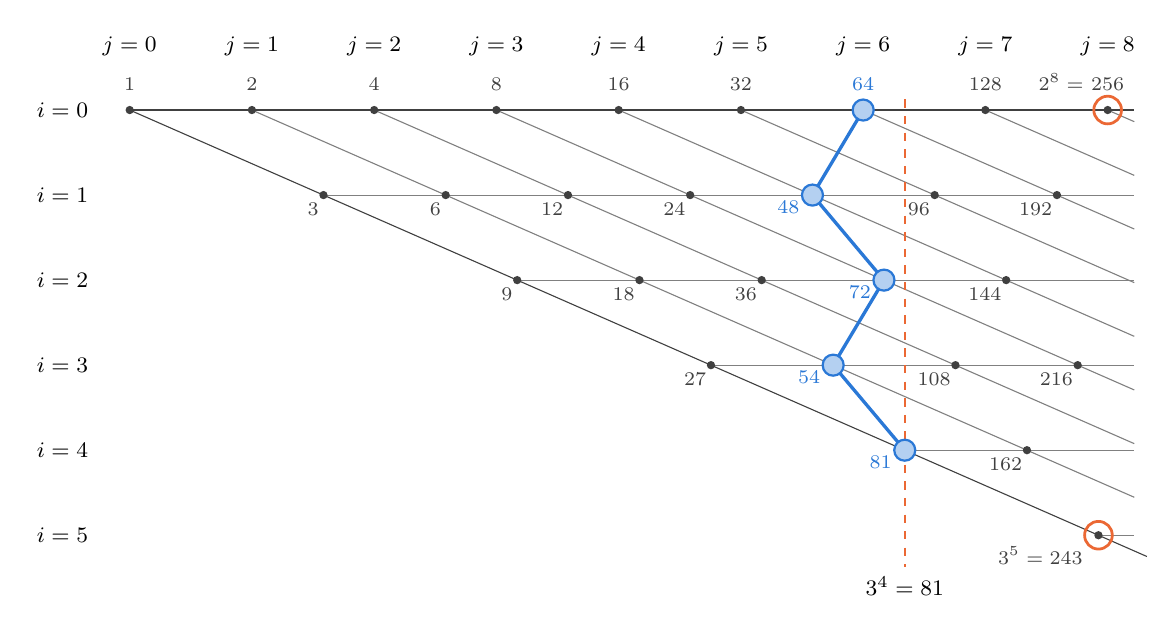
\begin{tikzpicture}\staircasefig\end{tikzpicture}
\caption{The first word \bw{11011010} of Order $5$ as a staircase on the slanted grid: its
odd steps at positions $0, 1, 3, 4, 6$ are the points $81$, $54$, $72$, $48$, $64$, and
$\rho = 319$. Each grid point $2^j 3^i$ carries its value. Dashed: the wall at $3^4$. Ringed: $3^5$ and $2^{p_2(5)} = 2^8$, whose
difference $13$ is $d_{23}$.}
\label{fig:staircase}
\end{figure}

\subsection*{The bounds on rho}

Every point of the staircase is at most $3^{n-1}$, so $\rho \le n\,3^{n-1}$
(\lean{rho\_le\_of\_admissible}); Chapter~\ref{sec:rhomax} finds the largest $\rho$, where
every point stands as far right as the wall allows. From below, $k_o \ge o - 1$ in every
word, so each point is at least $3^{n-o}\,2^{o-1}$ and
$\rho \ge \sum_{o} 3^{n-o}\,2^{o-1} = 3^n - 2^n$, with equality exactly for the words that
start with all their odd steps (\lean{three\_pow\_le\_rho\_add},
\lean{rho\_add\_eq\_three\_pow\_iff}). The staircase of such a word is the diagonal from
$3^{n-1}$ down to $2^{n-1}$.

\subsection*{The two ends}

The cycle point $x^* = \rho/d_{23}$ has $d_{23}(n) = 2^{p_2(n)} - 3^n$, a
difference of two $3$-smooth numbers: $3^n$ at the start of row $n$, and $2^{p_2(n)}$, the
first power of $2$ beyond it. A $3$-smooth number $2^j 3^i$ lies strictly between them
exactly when $1 \le i < n$, $j = p_2(n) - p_2(i)$ and the block factor of $i$ is above that
of $n$ (\lean{smooth\_between\_iff}). So none lies between them exactly when $n$ is an
upper record Order (\lean{upperRecord\_iff\_none\_between}): in
Figure~\ref{fig:staircase}, nothing lies between $243$ and $256$; for $n = 2$, the number
$12 = 2^2 \cdot 3$ lies between $9$ and $16$.

Walking up through the $3$-smooth numbers from $3^n$ to $2^{p_2(n)}$, each step is one of
the two of paper~2, Chapter~\ref{P2-sec:chain}: from $2^j 3^i$ the exponent of $3$ falls by
the last upper record Order $b \le i$, or rises by the last lower record Order $a$ with
$p_2(a) \le j + 1$ (\lean{smooth\_succ}). After a power of $3$ it is always the step down by
$b$ (\lean{smooth\_succ\_of\_pow\_three}); at an upper record Order $n$ that one step, with
$b = n$, goes from $3^n$ straight to $2^{p_2(n)}$.

\subsection*{Over the power series in $q$}
% Generation 80 (user, S36: B, C): TMonksQ; Monks' tables checked exactly in Python
% (_tmp/monks/monks_h_01.py, _02.py; all 20 rows of each table).

K.~G.~Monks~\cite{Monks2025} carries $T$ over to the power series in $q$ over the field with
two elements: for $A$ and $B$ with constant term $1$, $T_{A,B}(x) = x/q$ when $q$ divides
$x$, and $(Ax + B)/q$ otherwise; each $T_{A,B}$ is conjugate to $T$ by a map that keeps the
parities. The staircase goes with it. If $x$ has $n$ odd steps among its first $L$ steps,
the $o$-th at position $k_o$, then
\[
q^L\,T_{A,B}^L(x) = A^n x + B\rho_A, \qquad \rho_A = \sum_{o=1}^{n} A^{\,n-o}\,q^{\,k_o},
\]
the formula for $\rho$ with $2$ replaced by $q$ and $3$ by $A$, and no signs, as $1 + 1 = 0$
(\lean{X\_pow\_mul\_monksT\_iterate}). For $A = 1$ the map is the shift $\sigma$ (which
deletes the first coefficient) conjugated by $B$: $T_{1,B}(By) = B\,\sigma(y)$
(\lean{monksT\_one\_mul}). Monks lists the series that correspond to $x = 1, \dots, 20$
for $A = 1 + q$, $B = 1$ and for $A = 1$, $B = 1 + q^2$, and asks for a closed formula. For a
start $x$ that reaches $1$ after $L$ steps, $1$ corresponds to the point $B/(A + q^2)$ of the
$2$-cycle of $T_{A,B}$, so its series is $(q^L B/(A + q^2) + B\rho_A)/A^n$; for $A = 1$,
$B = 1 + q^2$ this is the polynomial $q^L + (1 + q^2)\sum_o q^{k_o}$, of degree $L$
(checked for all 20 rows of both tables). With the coefficients as binary digits, the second
table is OEIS A389685\index{OEIS!A389685}~\cite{OEIS_A389685}, the value at $q = 2$ of this
polynomial (checked for $n \le 10^4$). The closed formula is the orbit itself.

\nopagebreak

\begin{wordbox}
\boxhere{staircase}staircase\index{staircase@\termlink{staircase}{staircase}|textbf} & the $n$ terms $3^{n-o}\,2^{k_o}$ of $\rho$ of a word of Order $n$, one point in each row of the grid of the $3$-smooth numbers. \\
\boxhere{slanted}slanted grid\index{slanted grid@\termlink{slanted}{slanted grid}|textbf} & $2^j 3^i$ drawn at $j + i\log_2 3$ in row $i$: the points stand in the order of their values. \\
\boxhere{wall}wall\index{wall@\termlink{wall}{wall}|textbf} & the vertical line through $3^{n-1}$; a word is admissible when every point after the first lies left of it, and its length is $p_2(n)$.
\end{wordbox}

\section{The largest rho and the finite reduction}
\label{sec:rhomax}
% Generation 69: first text. Material (c) of Backlog 17: TRhoMax, TRhoSlack, TRhoMaxBound,
% TRhoMaxRecord, TRhoMaxCheck, TRhinCheck. Proved = in Lean where a name is given;
% Table 1 computed exactly (integers), the walk counts recounted outside Lean.

Paper~2 bounds $\rho$ by $n\,3^{n-1}$ for every admissible word of Order $n$, and so the
width identity needs checking only at class ids up to $\tau(n) = n\,3^{n-1}/d_{23}(n)$
(paper~2, Chapter~\ref{P2-sec:open}). This chapter replaces $n\,3^{n-1}$ by the largest
$\rho$ that an admissible word of Order $n$ really has, a sum of $3$-smooth numbers, and
shows that the finite reduction keeps its shape: its records are again exactly the upper
record Orders.

\subsection*{The largest rho}

\termhere{rhomax}In $\rho = \sum 3^{n-o}\,2^{k}$ the $o$-th odd step stands at position $k$. In an
admissible word the odd step that follows $m$ odd steps stands at a position $k$ with
$k + 1 \le p_2(m)$ (\lean{admissible\_step\_le}): before it the level is at least $1$.
Each term grows with its position, so $\rho$ is largest when every odd step stands as late
as it may, at $k = p_2(o - 1) - 1$. That gives
\[
\keysym{rhomax}{\rho_{\max}(n)} = \sum_{m < n} 3^{\,n-1-m}\,2^{\,p_2(m)-1},
\qquad \rho_{\max}(n + 1) = 3\,\rho_{\max}(n) + 2^{\,p_2(n)-1},
\]
and $\rho \le \rho_{\max}(n)$ for every admissible word of Order $n$
(\lean{rho\_le\_rhoMax}, \lean{rhoMax\_eq\_sum}). Every term is a $3$-smooth number: in the
grid of Chapter~\ref{sec:staircases}, each odd step stands as close to the line as
admissibility allows. The one admissible word with every odd step at its latest position is the first word
of Order $n$ (rank~$1$), and it is the only word that reaches the bound
(\lean{rho\_eq\_rhoMax\_iff}, \lean{rho\_lt\_rho\_firstWord}). For $n = 3$ the first word is
\bw{11010}, with odd steps at $0$, $1$ and $3$, and $\rho_{\max}(3) = 9 + 6 + 8 = 23$,
against $n\,3^{n-1} = 27$.

At a record Order the first word is an upper Christoffel word~\cite[Definition~1.1]{BerstelLRS2008}:
with $P = p_2(n)$ at an upper record Order $n$, and $P = p_2(n) - 1$ at a lower one, its $o$-th
odd step stands at $\lfloor (o-1)P/n \rfloor$, by $\lfloor iP/Q \rfloor + 1 = p_2(i)$ for a
record fraction $P/Q$ (Chapter~\ref{sec:a003586}); with $\bw{0}$ as $x$ and $\bw{1}$ as $y$
these $P$ letters are the upper Christoffel word of slope $n/(P - n)$
(\lean{take\_firstWord\_recordFrac}; $n$ and $P$ are coprime, \lean{RecordFrac.coprime}:
a common factor would give an earlier record), and at a lower record Order a $\bw{0}$ follows.
Below Order $200$ the first word has this form at no other Orders than these and $4$, $6$,
$24$, $36$, $48$, $106$, $159$, where $(p_2(n) - 1)/n$ is the record fraction of a lower record
Order, not in lowest terms, and the first $p_2(n) - 1$ letters a power of that Order's
Christoffel word (measured).

\termhere{slack}What the bound $n\,3^{n-1}$ gives away, its \keyterm{slack}{slack}, is a sum of the lower deficits
$2 \cdot 3^m - 2^{p_2(m)}$:
\[
2\,\bigl(n\,3^{n-1} - \rho_{\max}(n)\bigr) = \sum_{m < n} 3^{\,n-1-m}\,
  \bigl(2 \cdot 3^m - 2^{p_2(m)}\bigr)
\]
(\lean{rhoMax\_slack}; for $n = 3$: $0 + 6 + 2 = 8$). Two of its terms compare like
$(2 \cdot 3^m - 2^{p_2(m)})\,3^k$ and $(2 \cdot 3^k - 2^{p_2(k)})\,3^m$
(\lean{slackTerm\_lt\_iff}), and the term of $m$ is below every earlier one from $k = 1$ on
exactly when $m$ is a lower record Order (\lean{lowerRecord\_iff\_slackTerm}). So the upper
record Orders are where $d_{23}$ is smallest so far, the lower ones where a term of the slack is.

\subsection*{The finite reduction with the largest rho}

A class id $c$ of a word of Order $n$ drops at its end when $\rho < d_{23}\,c$, so only the
class ids with $d_{23}\,c \le \rho_{\max}(n)$ can fail:
\[
\text{the width identity} \iff
  \text{every class id } c > 1 \text{ with } d_{23}\,c \le \rho_{\max}(n) \text{ drops}
\]
(\lean{classDrops\_iff\_small\_rhoMax}). \termhere{W}Per Order, the class ids up to
\[
\keysym{W}{W(n)} = \Bigl\lfloor \frac{\rho_{\max}(n)}{d_{23}(n)} \Bigr\rfloor \le \lfloor \tau(n) \rfloor
\]
suffice, and a range check of every $x$ with $1 < x \le X$ gives the width identity at every
Order with $W(n) \le X$ (\lean{classDropsAt\_of\_widthMax},
\lean{classDropsAt\_of\_verifiedMax}, \lean{widthBoundMax\_le\_widthBound}).

\subsection*{The records}

The ratio $\rho_{\max}(n)/d_{23}(n)$, and its floor $W(n)$, are above their values at every
earlier Order exactly at the upper record Orders (\lean{upperRecord\_iff\_rmax},
\lean{upperRecord\_iff\_widthBoundMax}), as for $\tau$. Both factors of
\[
\frac{\rho_{\max}(n)}{d_{23}(n)} = \frac{\rho_{\max}(n)/3^n}{1/f(n) - 1}
\]
work the same way: $\rho_{\max}(n)/3^n$ grows with $n$ (\lean{three\_pow\_mul\_rhoMax\_le}), and
$1/f(n) - 1$ falls as the block factor $f(n)$ of paper~2, Chapter~\ref{P2-sec:chain}, rises. So a
later Order with a block factor at least as large has a ratio at least as large
(\lean{rmax\_le\_of\_le\_of\_blockFactor\_le}), and an upper record Order has a ratio above every
earlier one.

For the other direction, let $n$ be no upper record Order, $a$ the last upper record Order
below it and $b = n - a$. Then $p_2$ is additive at every split $a + j$ with $1 \le j \le b$,
and
\[
\rho_{\max}(a + b) = 3^b\,\rho_{\max}(a) + 2^{p_2(a)}\,\rho_{\max}(b)
  - 3^{\,b-1}\,2^{\,p_2(a)-1},
\qquad
d_{23}(a + b) = 3^b\,d_{23}(a) + 2^{p_2(a)}\,d_{23}(b)
\]
(\lean{rhoMax\_add}). Without the last term the ratio at $a + b$ would be a mediant of the
ratios at $a$ and $b$, with the weights $3^b$ and $2^{p_2(a)}$; the term takes it below. With
the ratio at $b$ at most that at $a$ (by induction), the ratio at $n$ is below that at $a$
(\lean{rmax\_add\_lt}). That the floor $W$ has the same records takes one more step: for
two Orders $c < n$ with $f(3) \le f(c) \le f(n)$, the ratio at $n$ is at least $1$ above
that at $c$ (\lean{rmax\_add\_one\_le}).

Table~\ref{tab:rhomax} puts $W(n)$ beside $\lfloor \tau(n) \rfloor$ at the upper record
Orders of paper~2's Table~\ref{P2-tab:tau}. With the last upper record Order $a$ up to $n$,
$W$ of every Order up to $n$ is at most $W(a)$ (\lean{widthBoundMax\_le\_of\_upperRecord}), so
a range check up to $W(a)$ gives the width identity at every Order up to $n$
(\lean{classDropsAt\_of\_verifiedMax\_record}). For the Orders below $10\,781\,274$ the range
check of paper~2 could have stopped at $W(190\,537) = 710\,220\,447\,737$ instead of
$984\,572\,779\,224$.

\begin{table}[htbp]
\centering
$\begin{array}{r r r r}
\toprule
n & p_2(n) & \lfloor \tau(n) \rfloor & W(n) \\
\midrule
3 & 5 & 5 & 4 \\
17 & 27 & 144 & 108 \\
41 & 65 & 1\,185 & 867 \\
306 & 485 & 99\,729 & 72\,058 \\
15\,601 & 24\,727 & 285\,814\,986 & 206\,178\,386 \\
47\,468 & 75\,235 & 1\,447\,674\,321 & 1\,044\,289\,613 \\
79\,335 & 125\,743 & 7\,216\,089\,270 & 5\,205\,340\,379 \\
190\,537 & 301\,994 & 984\,572\,779\,224 & 710\,220\,447\,737 \\
\bottomrule
\end{array}$
\caption{The bound of paper~2 and the bound with the largest $\rho$, at some upper record
Orders (exact).}
\label{tab:rhomax}
\end{table}

\subsection*{The bound from Rhin, checked to Order \texorpdfstring{$10^{60}$}{10\^{}60}}

Paper~2 cites Rhin's~\cite{Rhin1987} lower bound for $2^{p_2(n)} - 3^n$ as a hypothesis
(\lean{RhinBound}) and notes that Lean's kernel checks $3^n \le p_2(n)^2\,(2^{p_2(n)} - 3^n)$
for every $n \le 10^{60}$ (\lean{rhinBoundUpTo\_one\_two}). This is a finite check, and no
proof uses it; what is of interest is how it avoids the powers $3^n$ with $n$ near $10^{60}$.
In product form, with $Q = p_2(n)$, the bound reads $3^n\,(1 + Q^2) \le Q^2\,2^Q$. Between
upper record Orders the block factor stays at most its value at the last record $a$, and
$p_2$ does not fall; so the bound at $a$ gives it at every Order up to the next record
(\lean{rhinAt\_of\_record}, \lean{rhinBoundUpTo\_of\_records}). The upper record Orders are the
upper denominators of the walk down the Stern--Brocot tree towards $\log_2 3$ (paper~2,
Figure~\ref{P2-fig:tau}), and at each such fraction $p/n$ with $p = p_2(n)$ the check at the
fraction computes no power $3^n$ with $n > 100$: for $n \le 100$ it is exact, and otherwise it comes from a
bracket $3^K < 2^b$ with $K = 2^{400}$. Raised to the power $K$, the bound follows from
$b\,n + \lfloor K/\lfloor p^2/2 \rfloor \rfloor + 1 \le p\,K$, a comparison of numbers of at most
$181$ digits, by $(1 + p^2)^K \le 2^{\lfloor K/\lfloor p^2/2\rfloor\rfloor + 1}\,p^{2K}$
(\lean{rhinOK\_spec}, \lean{succ\_pow\_le}). The walk itself is certified with the same bracket:
$649$ steps until the sum of its two denominators passes $10^{60}$,
with $320$ upper record Orders among them (\lean{rhinWalk\_ok}, computed by the kernel).

\subsection*{The lower side, and the differences of powers of 2 and 3}
% Generation 76: PowDiff, PowDiffRhin, PowDiffWalk (namespace PowDiff); the seqfan thread
% on OEIS A363998 to A364001.

The Rhin check bounds the gap $2^{p_2(n)} - 3^n$ above $3^n$. The same walk, at its lower
fractions, bounds the gap $3^n - 2^{p_2(n)-1}$ below: with $Q = p_2(n)$,
\[
2^{\,Q-1}\,(1 + Q^2) \le Q^2\,3^n \qquad (1 \le n \le 10^{60})
\]
(\lean{lowAt\_upTo}). Between lower record Orders it carries over as the upper side does
between upper ones (\lean{lowAt\_of\_records}), and the walk checks the lower fraction of every
node with the same bracket (\lean{lowWalk\_ok}, computed by the kernel). With both sides, no
power of $2$ comes close to a power of $3$:
\[
\min(2^i, 3^j) \le p_2(j)^2\,\lvert 2^i - 3^j \rvert \qquad (1 \le j \le 10^{60})
\]
(\lean{min\_le\_of\_walk}), so a number $v = \lvert 2^i - 3^j \rvert$ with $j \le 10^{60}$ has
$i, j < B$ for every $B \ge 3$ with $(4B^2 + 1)\,v < 2^B$ (\lean{lt\_of\_walk}).

% Generation 76: PowDiffFar; generation 78: the walks to 10^200 in the tree, in four
% stretches each (PowDiffFarRhin1..4, PowDiffFarLow1..4, PowDiffFarCheck; as one walk each
% they took about an hour and 20 GB; the bracket ends from literal checkpoints, PowDiffFarBracket).
Nothing in these proofs depends on the bound $10^{60}$ but the walk itself: any walk at
$K = 2^m$ that checks every node until its denominators pass $N$ gives both sides up to
Order $N$ (\lean{rhinBoundUpTo\_of\_walk}, \lean{lowAt\_of\_walk},
\lean{min\_le\_of\_walks}). The bracket has to grow with $N$: a walk to $10^{100}$ needs
$m = 670$ and $1063$ steps, one to $10^{200}$ needs $m = 1330$ and $5839$ steps
(computed in integers, with the bracket from $2m + 3$ bits as in \lean{log2Lo}): in each
case $K = 2^m$ is just above $N^2$ ($m$ tried in steps of $10$). The kernel has run both
walks to $10^{200}$, each in four stretches (\lean{rhinBoundUpTo\_one\_two\_200},
\lean{lowAt\_upTo\_200}), from a bracket whose $1330$ squarings it checks in fourteen
chunks, each from the state before it written out (\lean{farLo200\_eq},
\lean{farHi200\_eq}); so
$\min(2^i, 3^j) \le p_2(j)^2\,\lvert 2^i - 3^j \rvert$ holds for $1 \le j \le 10^{200}$
(\lean{min\_le\_of\_walk\_200}).

These differences are the terms of OEIS A014121~\cite{OEIS_A014121} ($i, j \ge 0$) and
A363999~\cite{OEIS_A363999} ($i, j \ge 1$). Beyond $10^{200}$ the bound needs Rhin's, which
enters in integers, as the hypothesis \lean{RhinInt}: when $2^i$ and $3^n$ are within a
factor $2$ ($i \ge 2$), the smaller is at most $i^{14}\,\lvert 2^i - 3^n \rvert$. It follows
from Rhin's bound by $\min(a, b)\,\lvert \log(a/b) \rvert \le \lvert a - b \rvert$, and
assumes less. Under it a finite search decides every $v$ (\lean{isPowDiff\_iff\_searchB}).
Without any bound, a congruence sieve proves the first $3000$ terms of A014121, up to
$N = 328\,256\,967\,394\,000\,206\,715$, and the $2891$ terms of A363999 up to $N$
(\lean{a014121\_iff}, \lean{a363999\_iff}): modulo $M = 2^8\,3^3\,p_1 \cdots p_{13}$, with
the $13$ primes $5, 7, 13, \ldots, 1153$ at which the orders of $2$ and $3$ divide $288$ and
$1728$, the residue of $2^i - 3^j$ for $i \ge 8$, $j \ge 3$ is one of $288 \cdot 1728$, and
each of those within $N$ of $0$ is the residue of a term; as $2N < M$, the residue gives
the number. The cases $i < 8$ or $j < 3$ are checked directly.

\nopagebreak

\begin{wordbox}
\boxhere{rhomax}$\rho_{\max}(n)$\index{rho max@\termlink{rhomax}{$\rho_{\max}(n)$}|textbf} & the largest $\rho$ of an admissible word of Order $n$, reached by the first word only. \\
\boxhere{slack}slack\index{slack@\termlink{slack}{slack}|textbf} & $n\,3^{n-1} - \rho_{\max}(n)$, a sum of lower deficits. \\
\boxhere{W}$W(n)$\index{W(n)@\termlink{W}{$W(n)$}|textbf} & $\lfloor \rho_{\max}(n)/d_{23}(n) \rfloor$: the class ids of Order $n$ up to it decide the width identity there.
\end{wordbox}

\section{The drop as a congruence}
\label{sec:congruence}
% Generation 68: first text. Proved = in Lean where a name is given, otherwise on paper;
% measured = by enumeration of every admissible word of the Orders named.

A word $w$ of Order $n$ and length $L = p_2(n)$ has its class id $c$, its $\rho$ and its
$d_{23} = 2^L - 3^n$, and a member $x$ of its class drops at the end of the word exactly
when $x$ lies above the cycle point $x^* = \rho/d_{23}$ (paper~2,
Chapter~\ref{P2-sec:numbers}). The class id is fixed by congruences, one for each piece of
the word. This chapter asks whether those congruences carry the drop, and finds that
they restate it.

\subsection*{Pieces of a word}

For any two words $u$ and $v$ (not necessarily admissible), with $n_u$ odd steps among
$L_u$ steps, and so on,
\[
\rho(uv) = 3^{n_v}\rho(u) + 2^{L_u}\rho(v)
\]
(\lean{rho\_append}), and likewise $2^{L} - 3^{n}$ of $uv$ is $3^{n_v}(2^{L_u} - 3^{n_u})
+ 2^{L_u}(2^{L_v} - 3^{n_v})$. A number with the steps $uv$ has the steps $u$, and after
them the steps $v$: so the class id $c$ of $uv$ is congruent to the class id of $u$ modulo
$2^{L_u}$, and $T^{L_u}(c)$ is congruent to the class id $c_v$ of $v$ modulo $2^{L_v}$.

\subsection*{Not block by block}

An admissible word splits at its record lows into the blocks of its chain,
$w = \bw{1}\,B_1 \cdots B_k$ (paper~2, Chapter~\ref{P2-sec:chain}), and each block is an
admissible word of lower Order. In one sentence: after the first \bw{1}, each block is a
small, local drop that ends below where it began (by a factor between $1/2$ and $1$,
\lean{one\_lt\_deficitRatio}, \lean{deficitRatio\_le\_two}); the blocks use up the $3/2$ of
that first \bw{1}, and the word drops when that budget is spent (\lean{validOrders\_iff\_budget};
at most one \bw{0} follows the last block). One could hope that the drop of $w$ follows from the drops
of its blocks: that $c$, carried through the word, passes above the cycle point of each
block in turn. It does not, and the cycle point itself shows why. For $w = \bw{1100}$
($c = 3$, $x^* = 5/7$) the blocks are $\bw{10}$ (cycle point $1$) and $\bw{0}$ (cycle
point $0$). Started at $5/7$, the word reaches $11/7 > 1$ before its first block and
$10/7 > 0$ before its second: $5/7$ passes every block's test, and yet it does not drop,
it comes back. So no argument block by block can give the drop.

\subsection*{The bound of a split}

\termhere{splitbound}What the congruences do give is a bound, the \keyterm{splitbound}{bound of a split}. Split $w = uv$. As $T^{L_u}(c)$ is a positive
number in the class of $v$, it is at least $c_v$, the least one; and $T^{L_u}(c) =
(3^{n_u} c + \rho(u))/2^{L_u}$, so
\[
c \;\ge\; X_u = \frac{2^{L_u} c_v - \rho(u)}{3^{n_u}}.
\]
When $X_u > x^*$, the drop at $c$ follows. The bound has a plain meaning. The steps $u$
send the cycle point of $uv$ to the cycle point of the rotation $vu$, and so
\[
X_u > x^*(uv) \iff c_v > x^*(vu)
\]
(\lean{split\_bound\_iff}, from the identity \lean{split\_identity} in integers). And for
the split after the leading \bw{1}, $w = \bw{1}\,v$: when $3c + 1 \le 2^L$, the number
$T(c) = (3c+1)/2$ is at most $2^{L-1}$ and has the steps $v$, so $T(c) = c_v$
(\lean{classId\_tail\_eq\_tStep}), and the bound of this split is the drop at $c$ itself
(\lean{split\_one\_iff}). The class ids that could break the width identity are at most
$\lfloor n 3^{n-1}/d_{23} \rfloor$ (paper~2), and for every Order up to $3000$ these satisfy
$3c + 1 \le 2^L$ (computed exactly): there the congruence bound is the width identity in
other words.

Measured, on every admissible word of Orders $2$ to $12$: whenever some split at the end of
a block gives $X_u > x^*$, the split after the leading \bw{1} does. On Orders $2$ to $18$
only four words have no split that gives the drop: \bw{11010} and \bw{11100} (Order~$3$),
\bw{11110100} and \bw{11111000} (Order~$5$). All four have $3c + 1 > 2^L$, at Orders where
$d_{23}$ is small ($5$ and $13$).

\subsection*{The cycle points of the blocks}

Measured on Orders $1$ to $18$: the class id of $w$ lies above the cycle point of every
block of its chain. This does not follow from the drop of $w$: on Orders $2$ to $13$ the
cycle point of $w$ is often below that of a block (for every word of Orders $7$ and $12$).
Nor from the drops of the blocks, as $c$ is not always above the class ids of its blocks.
It does follow from a statement per block, measured on Orders $2$ to $31$ (from Order $14$
on by a walk over the prefixes): the class id of
the prefix $\bw{1}\,B_1 \cdots B_i$ lies above the cycle point of $B_i$, as $w$ and that
prefix have the same residue modulo $2^{L_P}$, $L_P$ the length of the prefix. But that
statement holds the drop of $B_i$ itself whenever $T^{L_u}$ of the prefix's class id is
the class id of $B_i$. So it is no easier than the width identity.

% Generation 76 (Backlog 11, A2): _keep/e2_block_index.py, Orders 2 to 21, exact.
By the index $i$ of the block, the statement gets easier fast. On Orders $2$ to $21$ the
smallest ratio of the class id of $\bw{1}\,B_1 \cdots B_i$ to the cycle point of $B_i$ is
\[
\tfrac{35}{23} \approx 1.52, \quad \tfrac{2015}{227} \approx 8.88, \quad
\tfrac{19643}{259} \approx 75.8, \quad \tfrac{13041}{5} \approx 2608, \quad
\tfrac{1700937}{5} \approx 340\,187
\]
for $i = 1, \ldots, 5$; the first three are reached at Orders $4$, $7$ and $12$, and stay the
smallest at every higher Order measured. The cycle point of a block is at most $W$ of its
Order, which grows like a power of the Order, while the class id of a longer prefix is fixed
by more bits. So the first block is where the statement is tight, and there it contains
the width identity: every admissible word $B$ is the first block of $\bw{1}\,B$, and when
$c$, the class id of $\bw{1}\,B$, has $3c + 1 \le 2^{1 + L_B}$, the class id of $B$ is
$T(c) > c$ (\lean{classId\_tail\_eq\_tStep}); so $c$ above the cycle point of $B$ gives the
drop of $B$. (On Order $14$ this holds for $5927$ of the $17\,637$ words.)

\nopagebreak

\begin{wordbox}
\boxhere{splitbound}bound of a split\index{bound of a split@\termlink{splitbound}{bound of a split}|textbf} & $X_u = (2^{L_u} c_v - \rho(u))/3^{n_u}$ for $w = uv$: the class id $c$ of $w$ is at least $X_u$.
\end{wordbox}

\section{The \texorpdfstring{$n$}{n}-th 3-smooth number, without the list}
\label{sec:a003586}
% Generation 69: first text. Material (b) of Backlog 17: TFloorSum, TBisect, TRecordFloor,
% TRecordWalk, TSmoothRank, TSmoothProgram, TSmoothProgramConv, TSternBrocotCert.
% The example (n = 51) computed with exact integers and checked against the sorted list.

The $n$-th $3$-smooth number $a(n)$ (OEIS A003586\index{OEIS!A003586}~\cite{OEIS_A003586}) can be found without listing the
$n - 1$ before it. The author's PARI program in that entry does it in two stages, with
$\log_2 3$ replaced by a fraction $P/Q$, and Lean proves the program right, in integers, for
every $n \ge 1$. It uses only what Chapters~\ref{sec:staircases} and~\ref{sec:rhomax} use:
the binary lengths $p_2(i)$ of the powers of $3$, and the record Orders.

\subsection*{Record fractions}

\termhere{recordfrac}Call $P/Q$ a \keyterm{recordfrac}{record fraction} when $Q$ is an upper record Order with $P = p_2(Q)$ or a
lower one with $P = p_2(Q) - 1$ (\lean{RecordFrac}). Such a fraction gives the binary lengths
by floors, $\lfloor iP/Q \rfloor + 1 = p_2(i)$ for $1 \le i < Q$
(\lean{div\_record\_add\_one}), and the number of powers of $3$ below $2^t$ as
$\lfloor tQ/P \rfloor + 1$ for $1 \le t < P$ (\lean{div\_record\_swap\_add\_one}).

\subsection*{The first stage: the number of binary digits}

\termhere{S}The $3$-smooth numbers with exactly $t$ binary digits are the $2^{t - p_2(i)}\,3^i$, one for
each power of $3$ below $2^t$. So the count \keysym{S}{$S(k)$} of the $3$-smooth numbers below $2^k$ is
$k$ plus a sum of floors $\lfloor tQ/P \rfloor$, a classical floor sum, computed by
Euclidean descent (\lean{floorSum\_eq}, \lean{smoothCount\_eq}); this is Mintz's count of
paper~2 at the powers of $2$. A bisection (\lean{bisect\_spec}) gives the number $B$ of
binary digits of $a(n)$, its rank $r = n - S(B-1)$ among the numbers of $B$ digits, and
their count $N = S(B) - S(B-1)$.

\subsection*{The second stage: the rank inside the class}

Inside the class of $B$ digits, $2^{B - p_2(i)}\,3^i$ for $i < N$, the numbers are sorted by
the block factor $f(i) = 3^i/2^{p_2(i)}$: below one of them lie the $3$-smooth numbers below
$2^{B-1}$ and those of the class with a smaller block factor
(\lean{card\_smoothBelowAt\_class}). With $u$ and $v$ the last lower and the last upper
record Order below $N$ (a walk from $(1, 1)$, \lean{recordWalk\_spec}), the block factor
rises along $i = k u \bmod (u + v)$, $k = 0, 1, \dots$, skipping $i \ge N$
(\lean{card\_blockFactor\_lt\_eq}, \lean{card\_mul\_mod\_lt}): the three-gap theorem. The
number of kept $i$ among the first $k$ is a difference of two floor sums
(\lean{classCount\_eq}), so a second bisection gives the $k$ of rank $r$, hence $i$, and
$j = B - 1 - \lfloor iP/Q \rfloor = B - p_2(i)$. The program returns $(j, i)$, and exactly
$n - 1$ of the $3$-smooth numbers lie below $2^j 3^i$ (\lean{smoothJI\_spec},
\lean{latticeOrd\_smoothJI}), for every record fraction $P/Q$ with $P > 2h$,
$h = 4 \cdot 2^{\lfloor \log_2(n)/2 \rfloor}$. The program computes floor sums of $P$, $Q$ and
Orders only: it forms no $3$-smooth number, not even $a(n)$.

For $n = 51$: $S(11) = 47$, so $B = 12$ and $r = 4$. The class of $12$ digits has $N = 8$
members, one for each power of $3$ below $2^{12}$; $u = 7$ and $v = 5$, and the sweep
$k \cdot 7 \bmod 12$ gives $0, 7, 2, (9), 4, (11), 6, 1, (8), 3, (10), 5$, the ones in
parentheses skipped: $2048$, $2187$, $2304$, $2592$, \dots{} in increasing order. The fourth
is $i = 4$, $j = 12 - p_2(4) = 5$: $a(51) = 2^5 \cdot 3^4 = 2592$.

\subsection*{Where the fraction comes from}

The PARI program takes $P/Q$ from \texttt{bestappr}, which returns a convergent. Every
semiconvergent $p/n$ of $\log_2 3$ is a record fraction (\lean{recordFrac\_of\_semiconv}), so
is every convergent (\lean{recordFrac\_conv}), and with one whose numerator exceeds $2h$ the
program returns the exponents of $a(n)$ (\lean{latticeOrd\_smoothJI\_conv}). That
\texttt{bestappr} returns convergents of $\log_2 3$, and not of a nearby number, is a matter
of PARI's working precision, outside the proof. Without it, the fraction comes from the
Stern--Brocot walk towards $\log_2 3$ in integers: a bracket $2^a \le 3^K < 2^b$ for
$K = 2^m$, from fixed-point squaring, decides each mediant $p/n$ by $pK \le an$ (below) or
$bn \le pK$ (above), and every step it decides is a step of the true walk, so the walk ends
at record fractions (\lean{sbCertStep\_eq}, \lean{exists\_sbCert}). For every large $m$ the
walk passes any numerator (\lean{exists\_lt\_walkAt}), and the program with the least such $m$
returns the exponents of $a(n)$ for every $n \ge 1$ (\lean{latticeOrd\_smoothJIFind}): no
convergent is assumed. Shanks~\cite{Shanks1954} computed the continued fraction of a
logarithm from the powers alone, and Jackson and Matthews~\cite{JacksonMatthews2002} with
floor and ceiling in fixed point, where the agreement of the two makes a partial quotient
likely, not certain; here every step the bracket decides is proved.

\nopagebreak

\begin{wordbox}
\boxhere{recordfrac}record fraction\index{record fraction@\termlink{recordfrac}{record fraction}|textbf} & $P/Q$ with $Q$ an upper record Order and $P = p_2(Q)$, or a lower one and $P = p_2(Q) - 1$. \\
\boxhere{S}$S(k)$\index{S(k)@\termlink{S}{$S(k)$}|textbf} & the number of $3$-smooth numbers below $2^k$. \\
A003586\index{OEIS!A003586} & the $3$-smooth numbers in the OEIS.
\end{wordbox}

\section{The minimal class ids}
\label{sec:minimal}
% Generation 69: first text. Backlog 5; the History (generation 35, the negatives). Terms:
% the run to 400 (_tmp/a122442_search_03.out) had a(1..397) at the time of writing:
% update the count when the run ends. Left out: the measured heuristics of generation 35
% (not wanted). Generation 76: the complexity placement (Manders-Adleman 1978, Theorem 2;
% Mahaney 1982, Theorem 3.1 and Corollary 3.6; both PDFs in _keep/).

The smallest class id of each Order is OEIS A122442\index{OEIS!A122442}~\cite{OEIS_A122442}, with $5$ in the place of the class id
$1$ of Order~$1$: $a(n)$ is the smallest $x > 1$ whose drop comes at Order $n - 1$, so
$2, 5, 3, 11, 7, 39, 287, 231, \dots$ (paper~2, Chapter~\ref{P2-sec:numbers}). The entry
defines it by the dropping time, and it is the smallest class id of each Order where the
class id drops at the end of its own word, which is checked for every term below.

\subsection*{The scan}

\termhere{scan}The terms are found by a \keyterm{scan}{scan}. A
residue $x \bmod 2^W$ fixes the first $W$ steps of $x$; the residues with no admissible prefix within
those $W$ steps are kept, $3\,524\,586$ of them for $W = 28$; for the others the residue fixes
the Order. The kept
residues are then taken in increasing order of $x$, round by round, and each $x$ is followed
to its drop. As $x$ grows, a term is final as soon as it is found. Each term is checked when
it is written: its trajectory reaches its drop exactly at Order $n - 1$, and the drop value
is below $a(n)$. The terms $a(1)$ to $a(397)$ are computed so; the last of them is
$a(397) = 87\,784\,734\,829\,927$.

\subsection*{Why not a smarter search}

The class id of a word is fixed by a congruence modulo $2^L$, and that is easy: for one
word, $c \equiv -\rho\,3^{-n} \pmod{2^L}$ (Chapter~\ref{sec:congruence}). The hard part is
the choice of the word. Two attempts to choose it well, and why they fail:
\begin{itemize}
\item \emph{Local moves.} Moving the $r$-th odd step of a word from position $k$ to $k'$,
  keeping it admissible, changes $\rho$ by $3^{n-r}\,2^k\,(2^{k'-k} - 1)$, a local change;
  but it changes the class id by $-3^{-r}\,2^k\,(2^{k'-k} - 1)$ modulo $2^L$: the bits below
  $k$ stay, all the bits above can change. A descent by such moves is a restart above
  the first changed position.
\item \emph{A solver.} An SMT encoding (M.~Winkler's suggestion: Boolean steps, the
  levels, the Order, the least $x$ by bisection on a bound) reproduces $a(n)$ and its words
  for Orders $1$ to $25$ (measured). Its bit-vector solver fixes the low bits of $x$ first,
  which is the scan by residues again.
\end{itemize}

\subsection*{Where the problem sits}

In terms of the residues, $c \equiv -\sum_o 3^{-o}\,2^{k_o} \pmod{2^L}$, with the $o$-th odd
step at position $k_o$: the smallest class id of an Order asks for a choice of positions,
under admissibility, that makes a modular sum small. Problems of this shape can be hard
because of the bound. Manders and Adleman~\cite{MandersAdleman1978} showed that deciding
whether $x^2 \equiv \alpha \pmod{\beta}$ has a solution with $0 \le x \le \gamma$ is
NP-complete (their Theorem~2), also when $\beta$ is given in factored form; without the
bound, square roots modulo a factored $\beta$ are found in random polynomial time. Here the congruence for one word is
linear and its least solution is the residue itself; what is left is the choice of the
word, and no reduction from an NP-complete problem to it is known.

There is also a reason why such a reduction is unlikely. Per Order there is one answer,
$a(n)$, so with $n$ written in unary the set of triples $(1^n, i, b)$ with bit $i$ of $a(n)$
equal to $b$ has only polynomially many strings of each length: it is sparse. By
Mahaney's theorem~\cite{Mahaney1982} (Theorem~3.1 and Corollary~3.6 there), if an
NP-complete set is many-one reducible in polynomial time to a sparse set, then
$\mathrm{P} = \mathrm{NP}$. So computing $a(n)$ is not NP-hard in that sense unless
$\mathrm{P} = \mathrm{NP}$. Neither statement says how hard $a(n)$ is; both say only that
the hardness, if any, is not of the usual kind.

\nopagebreak

\begin{wordbox}
\boxhere{scan}scan\index{scan@\termlink{scan}{scan}|textbf} & the odd $x$ taken in increasing order over the residues modulo $2^W$ with no admissible prefix in $W$ steps, each followed to its drop. \\
A122442\index{OEIS!A122442} & the smallest class id of each Order, in the OEIS.
\end{wordbox}

\section{Three letters: the stop of A324245}
\label{sec:three}
% Generation 70: first text. the History, generation 37; OEIS/a349414_variant_01.py, rerun
% for every odd k < 2^22 and the count to M = 16; the least starts recomputed (k < 2^22).
% Generation 71: proved = in Lean (TUds, TUdsDrop, TUdsCount). The shares of the stops by D and by S are
% left out (not wanted). The drafts A900001 to A900003 (postponed by the user) are not cited.

\termhere{letters}Papers~1 and~2 play a game with two letters. OEIS A324245\index{OEIS!A324245}~\cite{OEIS_A324245}, the map of Vaillant
and Delarue~\cite{VaillantDelarue2019} (paper~2, Chapter~\ref{P2-sec:fast}), has three \keyterm{letters}{letters}. It acts on $n$; on the odd number $k = 2n + 1$ it reads
\[
\mathtt{U}\colon k \equiv 3 \pmod 4 \mapsto \tfrac{3k+1}{2}, \qquad
\mathtt{D}\colon k \equiv 1 \pmod 8 \mapsto \tfrac{3k+1}{4}, \qquad
\mathtt{S}\colon k \equiv 5 \pmod 8 \mapsto \tfrac{k-1}{4}.
\]
The steps $\mathtt{U}$ and $\mathtt{D}$ go from $k$ to the next odd value of its path
under $T$. The step $\mathtt{S}$ does not: it replaces $k$ by the smaller odd number
$(k-1)/4$, which has the same next odd value, as $3\,(k-1)/4 + 1 = (3k+1)/4$. \termhere{stop}\termhere{M}\termhere{letterword}Follow $k$ by
these steps and \keyterm{stop}{stop} at the first value below $k$; let \keysym{M}{$M$} be the number of steps
$\mathtt{U}$ and $\mathtt{D}$ before the stop. For $k = 7$ the steps are
$7 \to 11 \to 17 \to 13 \to 3$, its \keyterm{letterword}{letter word} is $\mathtt{UUDS}$, and $M = 3$; for $k = 9$ one
step $\mathtt{D}$ goes to $7$, and $M = 1$.

\subsection*{The stop and the drop}

Before the stop every odd value reached is at least $k$, and the odd values of the path of
$k$ under $T$ are among them, in order. A stop by $\mathtt{D}$ is a step of that path: its
value is the first odd value of the path below $k$, and $M$ is the Order of the drop of
$k$. \termhere{merge}A stop by $\mathtt{S}$ is not: the path of $k$ under $T$ is still at or above $k$, and
from the stop value on it goes the same way, a \keyterm{merge}{merge} before the drop. So $M$ is at most the
Order of the drop, with equality exactly when the stop is by $\mathtt{D}$ (\lean{le\_order\_of\_isUdsStop}, \lean{isUdsStop\_of\_S}; checked
for every odd $k < 2^{22}$). The number $7$ drops at Order~$4$, to $5$, one odd step after
its merge with the path of $3$.

\subsection*{The words}

Write $\mathtt{U}$ as \bw{1}, $\mathtt{D}$ as \bw{10} and $\mathtt{S}$ as \bw{00}. The
letters multiply $k$ by about $3/2$, $3/4$ and $1/4$: the factors of the bits of a word of
paper~2. After a prefix of the letters the value is $P\,k + c$, with $P$ the product of the
factors and $c$ fixed by the prefix, so for all large $k$ of a class the stop comes at the
first prefix with $P < 1$ (\lean{isUdsStop\_iff\_of\_large}). It does so for every odd $k < 2^{22}$ (measured); whether
it does for every $k$ is open. At the last letter of a class that stops by $\mathtt{D}$ it
follows from the width identity of the word at which the class drops (\lean{ClassDrops};
paper~2, Chapter~\ref{P2-sec:open}).

By the product rule the bits of the letters up to the stop are an admissible word of
Order~$M$, or one followed by \bw{0}. A \bw{1} followed by $z$ zeros splits in exactly one
way into letters: $\mathtt{U}$ and $z/2$ letters $\mathtt{S}$ when $z$ is even,
$\mathtt{D}$ and $(z-1)/2$ letters $\mathtt{S}$ when $z$ is odd. The first product below $1$
falls at the end of an admissible word or one bit later, and both occur for every admissible
word. So for $m \ge 1$ there are $2\,\mathrm{A100982}(m)$\index{OEIS!A100982}~\cite{OEIS_A100982} letter words with $M = m$
(paper~2, Chapter~\ref{P2-sec:count}), $\mathrm{A100982}(m)$ of them fixing $k$ modulo
$2^{p_2(m)+1}$ and as many modulo $2^{p_2(m)+2}$ (\lean{card\_udsStopSet}, \lean{udsWord\_class}; counted for $m \le 16$). For $k = 7$
the bits are \bw{111000}, the admissible word \bw{11100} of Order~$3$ followed by \bw{0}.
These bits need not be the word of $k$: in the letters, the steps $\mathtt{S}$ of an odd
value come before its $\mathtt{U}$ or $\mathtt{D}$.

The least odd $k$ with $M = m$, for $m = 1, \dots, 15$:
$3$, $11$, $7$, $39$, $95$, $155$, $191$, $127$, $603$, $359$, $239$, $159$, $639$, $283$, $743$ (measured, $k < 2^{22}$).
For $m = 1$ to $4$, $7$, $8$ and $11$ to $14$ this is the least $x$ that drops at Order
$m + 1$ (Chapter~\ref{sec:minimal}).

\nopagebreak

\begin{wordbox}
\boxhere{letters}U, D, S\index{UDS@\termlink{letters}{U, D, S}|textbf} & the three steps on odd $k$: $(3k+1)/2$ for $k \equiv 3 \pmod 4$, $(3k+1)/4$ for $k \equiv 1 \pmod 8$, $(k-1)/4$ for $k \equiv 5 \pmod 8$. \\
\boxhere{stop}stop\index{stop@\termlink{stop}{stop}|textbf} & the first value below $k$ reached by the letters. \\
\boxhere{letterword}letter word\index{letter word@\termlink{letterword}{letter word}|textbf} & the letters of $k$ up to its stop; in bits \bw{1}, \bw{10}, \bw{00}. \\
\boxhere{M}$M$\index{M@\termlink{M}{$M$}|textbf} & the number of letters $\mathtt{U}$ and $\mathtt{D}$ up to the stop. \\
\boxhere{merge}merge\index{merge@\termlink{merge}{merge}|textbf} & a stop by $\mathtt{S}$: the stop value joins the path of $k$ under $T$ before its drop. \\
A100982\index{OEIS!A100982} & the number of admissible words of each Order, in the OEIS. \\
A324245\index{OEIS!A324245} & the map of the three letters, on $n = (k-1)/2$, in the OEIS.
\end{wordbox}

\section{The ruler gap}
\label{sec:ruler}
% Generation 69: first text. Material (a) of Backlog 17; item 10. SmoothRuler, TRulerRecord,
% TRulerDeficit, TRulerPair, TRulerCheck. Stopped by the user at rulerGap_iff_pairs (the
% finite check was his request); this chapter states what is there and adds nothing.

This chapter is an open statement on neighbouring $3$-smooth numbers, with its reductions.
Papers~1 and~2 do not use it, and nothing in this paper rests on it.

\subsection*{The statement}

\termhere{ruler}\termhere{rulergap}Draw the $3$-smooth numbers on a \keyterm{ruler}{plain ruler}: $v$ at distance $v$ from the left, in the row
of its number of factors $3$. Let $a < b$ be neighbours among them. A second step with the
same factor would land at $b^2/a$; the straight line from $a$ through $b$, continued over
the same number of rows, arrives at $2b - a$, which is before it
(\lean{line\_falls\_short}). The \keyterm{rulergap}{ruler gap} says that no $3$-smooth number lies
strictly between $2b - a$ and $b^2/a$ (\lean{RulerGap}). For $a = 8$, $b = 9$ the gap is
from $10$ to $81/8$. Under the ruler gap a $3$-smooth number lies before the second step
exactly when it lies at or before the end $2b - a$ of the line
(\lean{rule\_iff\_of\_rulerGap}). The same rule with the place where the continued line
meets row $0$ is false: from $3^{11}$ the step to $2^8 \cdot 3^6$ is to a neighbour, its
line meets row $0$ at $197\,996 + 2/5$, and the second step of that factor lands at
$2^{16} \cdot 3$, before that place (\lean{border\_rule\_fails}).

\subsection*{In exponents and record Orders}

The statement is one on exponents only (\lean{rulerGap\_iff\_ordersGap}). A step between
neighbours that raises the exponent of $2$ is a step of an upper record Order $b$, by the
factor $2^{p_2(b)}/3^b$; one that raises the exponent of $3$ is a step of a lower record
Order $a$, by $3^a/2^{p_2(a)-1}$ (\lean{stepAt\_two\_three\_iff},
\lean{stepAt\_three\_two\_iff}; these are the two steps of Chapter~\ref{sec:staircases}), and
the ruler gap is a statement on those steps (\lean{rulerGap\_iff\_records}). For a step of
an upper record Order $b$, a number in its gap is one more factor $3^v/2^u$ with
$u + 1 = p_2(v)$, where $b$ and $v$ split at $K = b + v$, $p_2(K) + 1 = p_2(b) + p_2(v)$,
and
\[
1 - f(K) < \bigl(1 - f(b)\bigr)^2
\]
for the block factor $f$ (\lean{gapAt\_two\_three\_iff\_deficit}); the lower record Orders
have their own inequality of this kind. So the ruler gap is the failure of these deficit
inequalities wherever the step is due (\lean{rulerGap\_iff\_deficit}), and the windows where
a step is due end at the next record Order. Over each window the block factor is extreme at
one record Order $c$, so the ruler gap is one inequality per pair of neighbouring record
Orders $b < b'$, at the largest upper record Order $c \le b + b'$, and likewise for the lower
ones (\lean{rulerGap\_iff\_pairs}). In words: the deficit $1 - f$ at such a $c$ is not below
the square of the deficit at $b$. That is a statement on how closely the fractions on the
Stern--Brocot walk approach $\log_2 3$, and it is open.

\subsection*{The finite check}

Lean's kernel checks the pair inequalities for every pair of neighbouring record Orders up
to $10^{60}$ (\lean{upperPairs\_upTo}, \lean{lowerPairs\_upTo}), with the certified walk of
Chapter~\ref{sec:rhomax}, here at $K = 2^{500}$ (\lean{rulerUpWalk\_ok}, \lean{rulerLowWalk\_ok}).
With an upper and a lower record Order between $10^{59}$ and $10^{60}$
(\lean{exists\_records\_between}), the ruler gap holds for every exponent of $2$ and every
exponent of $3$ up to $10^{59}$ (\lean{rulerGapUpTo\_ten\_pow}). This is a finite check; the
ruler gap itself stays open.

\nopagebreak

\begin{wordbox}
\boxhere{ruler}plain ruler\index{plain ruler@\termlink{ruler}{plain ruler}|textbf} & $v$ drawn at distance $v$, in the row of its number of factors $3$. \\
\boxhere{rulergap}ruler gap\index{ruler gap@\termlink{rulergap}{ruler gap}|textbf} & for neighbouring $3$-smooth numbers $a < b$: none lies strictly between $2b - a$ and $b^2/a$; open (\lean{RulerGap}).
\end{wordbox}

\section{What is left out}
\label{sec:leftout}
% Generation 70: first text. 3x-1: one remark, that it is left out, and why (user,
% generation 67). "Shares and ratios" decided in generation 83 (S33; a rule of the project:
% no shares or ratios in the papers); "Other multipliers" decided in generation 78 (below).

\subsection*{The map $3x - 1$}

On the negative numbers $T$ is the map $x \mapsto (3x - 1)/2$ for odd $x$, $x/2$ for even
$x$, with the sign turned. There the drop has a plain answer: $5 \to 7 \to 10 \to 5$ never
falls below $5$. Compared once with $T$ word by word, it showed the change of sign only, no link between
the classes (measured). It says nothing on the drop under $T$, and this paper leaves it out.

\subsection*{Shares and ratios}

Shares, such as how many of the starts of Chapter~\ref{sec:three} stop by $\mathtt{D}$, and
ratios seen on a range are not statements that hold for every number. They are left out.

\subsection*{Other multipliers}
% Generation 76 (B1): TBracketCountQ, TChainParseQ, TBracketDropQ; the measurement
% _keep/q_family_measure_01.py (_tmp/q_family_measure_01.out), Orders 1 to 10, exact.
% Generation 78 (user): cut to one sentence; the q = 5, 7, 9 measurement and the q = 9
% counts are out of the paper (the History, generation 77).

Other odd multipliers $q \ge 3$ are left out: paper~2 proves its chain decomposition and
sweeps for every odd $q$, as in M.~Winkler's~\cite{Winkler2026b}, and the lean-files
\lean{TBracketCountQ}, \lean{TChainParseQ} and \lean{TBracketDropQ} carry the rest of that
chapter over to every odd $q$.

\appendix
\section{The Lean formalization}
\label{app:lean}
% Generation 70: first text. The modules of the Lean names this paper cites, by chapter;
% every name mapped to its module by grep in generation 70 (82 names, 29 modules); generation 71: Ch. 8 in Lean (5 names, 3 modules); generation 76: the PowDiff files (Ch. 3); generation 84: TChristoffel (Ch. 3).

The Lean names this paper cites are proved in the Lean~4 project \lean{AcceleratedCollatz}
of papers~1 and~2 (paper~2, Appendix~\ref{P2-app:lean}), without \texttt{sorry}; open
statements and theorems taken from the literature enter as named hypotheses
(\lean{ClassDrops}, \lean{RulerGap}, \lean{RhinBound}, \lean{RhinInt}). Table~\ref{tab:lean3} lists the
lean-files by chapter; the names of the \lean{PowDiff} files are in the namespace \lean{PowDiff}. Chapter~\ref{sec:minimal} is computed, not formalized.

\begin{table}[htbp]
\centering
\footnotesize
\begin{tabular}{@{}l>{\raggedright\arraybackslash}p{0.40\linewidth}>{\raggedright\arraybackslash}p{0.45\linewidth}@{}}
\toprule
Ch. & lean-file & content \\
\midrule
1, 2 & \lean{TRho$\{$Bound,Lower$\}$}, \lean{TSmooth$\{$Between,Next,Place,Succ$\}$},
  \lean{TStaircase}, \lean{TWidth}, \lean{TMonksQ}
  & staircases, the bounds on $\rho$, the $3$-smooth numbers in order and between $3^n$
  and $2^{p_2(n)}$, the width identity, $\rho$ over the power series in $q$ \\
3 & \lean{TChristoffel}, \lean{TRhin$\{$Bound,Check$\}$}, \lean{TRho$\{$Max,Slack$\}$},
  \lean{TRhoMax$\{$Bound,Check,Record$\}$}
  & the largest $\rho$, the first word as a Christoffel word, its slack, the finite
  reduction and its records, the Rhin check \\
3 & \lean{PowDiff$\{$,Far,Rhin,Walk$\}$},
  \lean{PowDiffFar$\{$Bracket,Check,Nodes$\}$},
  \lean{PowDiffFar$\{$Low,Rhin$\}\{$1..4$\}$}
  & the lower side to $10^{60}$ and both sides to $10^{200}$, the differences $\lvert 2^i - 3^j \rvert$ (A014121, A363999) \\
4 & \lean{TCongruenceSplit}
  & $\rho$ of a concatenation, the bound of a split \\
5 & \lean{TBisect}, \lean{TFloorSum}, \lean{TRecord$\{$Floor,Walk$\}$},
  \lean{TSmooth$\{$Program,ProgramConv,Rank$\}$}, \lean{TSternBrocotCert}
  & the A003586 program \\
7 & \lean{TUds$\{$,Count,Drop$\}$}
  & the three letters: the stop and the drop, the stop for large $k$, the classes, the count \\
8 & \lean{SmoothRuler}, \lean{TRuler$\{$Check,Deficit,Pair,Record$\}$}
  & the ruler gap, its reductions and the finite check \\
9 & \lean{TBracketCountQ}, \lean{TChainParseQ}, \lean{TBracketDropQ}
  & every odd $q$: the bracket words, the parse, the brackets and the map $qx + 1$ \\
\bottomrule
\end{tabular}
\caption{The lean-files of this paper, by chapter; braces group names as in a shell, so
\lean{TRuler$\{$Check,Pair$\}$} is \lean{TRulerCheck} and \lean{TRulerPair}.}
\label{tab:lean3}
\end{table}

\begin{thebibliography}{99}
\bibitem{BerstelLRS2008} J.~Berstel, A.~Lauve, C.~Reutenauer and F.~V. Saliola,
  \emph{Combinatorics on Words: Christoffel Words and Repetitions in Words}, CRM Monograph
  Series~27, Amer.\ Math.\ Soc., Providence, 2008.
\bibitem{JacksonMatthews2002} T.~Jackson and K.~Matthews, \emph{On Shanks' algorithm for
  computing the continued fraction of $\log_b a$}, J. Integer Sequences \textbf{5} (2002),
  Article 02.2.7.
\bibitem{Mahaney1982} S.~R. Mahaney, \emph{Sparse complete sets for NP: solution of a
  conjecture of Berman and Hartmanis}, J.\ Comput.\ System Sci.\ \textbf{25} (1982),
  130--143.
\bibitem{MandersAdleman1978} K.~L. Manders and L.~Adleman, \emph{NP-complete decision
  problems for binary quadratics}, J.\ Comput.\ System Sci.\ \textbf{16} (1978), 168--184.
\bibitem{Mintz1981} D.~J. Mintz, \emph{2,3 sequence as binary mixture}, Fibonacci
  Quart.\ \textbf{19} (1981), 351--360.
\bibitem{Monks2025} K.~G. Monks, \emph{On $q$-analogs of the $3x + 1$ dynamical system},
  J. Integer Sequences \textbf{28} (2025), Article 25.6.8.
\bibitem{OEIS_A003586} OEIS Foundation Inc., \emph{Sequence A003586},
  \url{https://oeis.org/A003586}.
\bibitem{OEIS_A014121} OEIS Foundation Inc., \emph{Sequence A014121},
  \url{https://oeis.org/A014121}.
\bibitem{OEIS_A100982} OEIS Foundation Inc., \emph{Sequence A100982},
  \url{https://oeis.org/A100982}.
\bibitem{OEIS_A122442} OEIS Foundation Inc., \emph{Sequence A122442},
  \url{https://oeis.org/A122442}.
\bibitem{OEIS_A324245} OEIS Foundation Inc., \emph{Sequence A324245},
  \url{https://oeis.org/A324245}.
\bibitem{OEIS_A363999} OEIS Foundation Inc., \emph{Sequence A363999},
  \url{https://oeis.org/A363999}.
\bibitem{OEIS_A389685} OEIS Foundation Inc., \emph{Sequence A389685},
  \url{https://oeis.org/A389685}.
\bibitem{Rhin1987} G.~Rhin, \emph{Approximants de Pad\'e et mesures effectives
  d'irrationalit\'e}, S\'eminaire de Th\'eorie des Nombres, Paris 1985--86,
  Progr.\ Math.\ 71, Birkh\"auser, Boston, 1987, 155--164.
\bibitem{Shanks1954} D.~Shanks, \emph{A logarithm algorithm}, Math.\ Tables Aids Comput.\
  \textbf{8} (1954), 60--64.
\bibitem{VaillantDelarue2019} N.~Vaillant and P.~Delarue, \emph{The hidden face of the
  $3x+1$ problem. Part I: Intrinsic algorithm} (2019); linked from OEIS A324245.
\bibitem{Winkler2026b} M.~Winkler, \emph{Admissible $qx+1$ sequences,
  semiconvergents, and rational Catalan numbers}, arXiv:2609.22303 (2026).
\bibitem{Paper1} Ruud H.G. van Tol, \emph{Collatz, but stop at the drop; Now with less
  noise} (2026), \url{https://doi.org/10.5281/zenodo.23631044}.
\bibitem{Paper2} Ruud H.G. van Tol and Mike Winkler, \emph{Collatz, but stop at the drop;
  A game with two letters: the proofs} (2026), \url{https://doi.org/10.5281/zenodo.23631547}.
\end{thebibliography}

\printindex

\end{document}
